\documentclass[a4paper]{article}
\usepackage[T1]{fontenc}
\usepackage[utf8]{inputenc}
\usepackage[english]{babel}

\usepackage{amsmath}
\usepackage{amssymb}
\usepackage{a4wide}
\usepackage{dsfont}
\usepackage{lmodern}
\usepackage{listings}
\usepackage{graphicx}
\usepackage{float}

\setlength{\parindent}{0pt}

\title{\textbf{Assignment 1} \\ \small Statistical Methods for Machine Learning }
\author{\textbf{Group members}\\
        Ásbjørn Viderø Jøkladal\\
        Martin Holm Cservenka\\
        Tue Haulund}
\date{17\textsuperscript{th} of February, 2015}		

%=======================================================================
\begin{document}
\maketitle
\tableofcontents
\newpage
%=======================================================================

\section{Probability and Parameter Estimation}
\subsection{Univariate Gaussian Distributions}
Figure~\ref{fig:distributions} shows the 1-dimensional Gaussian density function for the parameter values $(\mu, \sigma) = (-1, 1), (0, 2) \text{ and } (2, 3)$.

\begin{figure}[H]
  \centering
  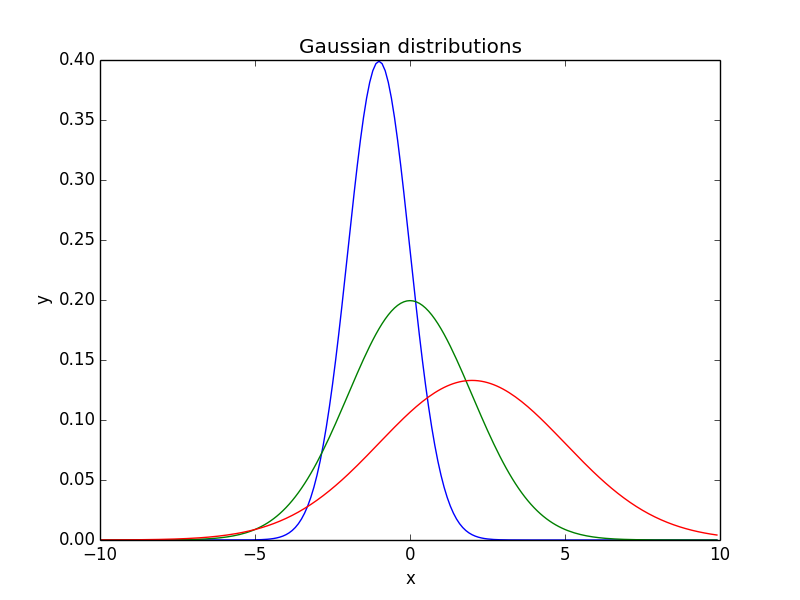
\includegraphics[width=.7\linewidth]{figures/distributions.png}
  \caption{Gaussian density function for the three sets of parameters.}
  \label{fig:distributions}
\end{figure}

\subsection{Sampling from a Multivariate Gaussian Distribution}
Figure~\ref{fig:samples} shows a plot of the generated data set.

\begin{figure}[H]
  \centering
  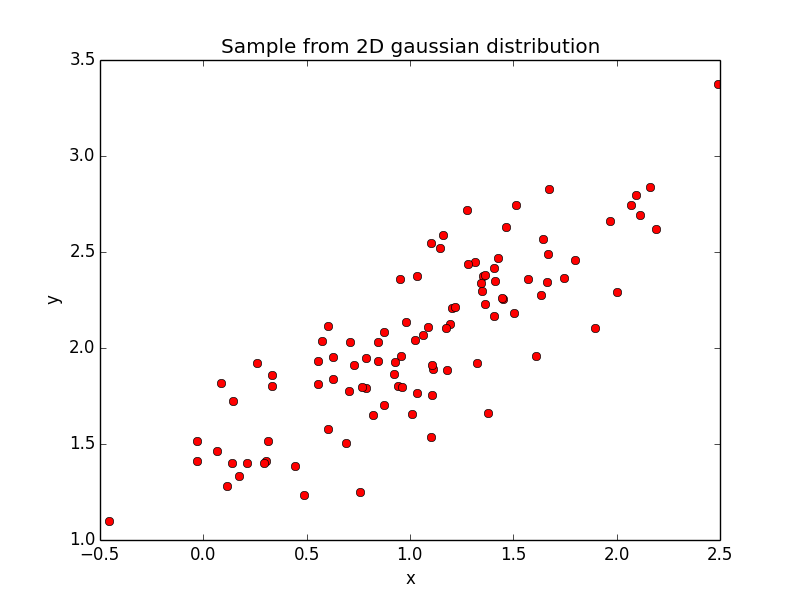
\includegraphics[width=.7\linewidth]{figures/samples.png}
  \caption{Plot of the generated data set.}
  \label{fig:samples}
\end{figure}

\subsection{Means}
Figure~\ref{fig:samples_with_mean} shows the sample mean and the distribution mean together with the data set.

\begin{figure}[H]
  \centering
  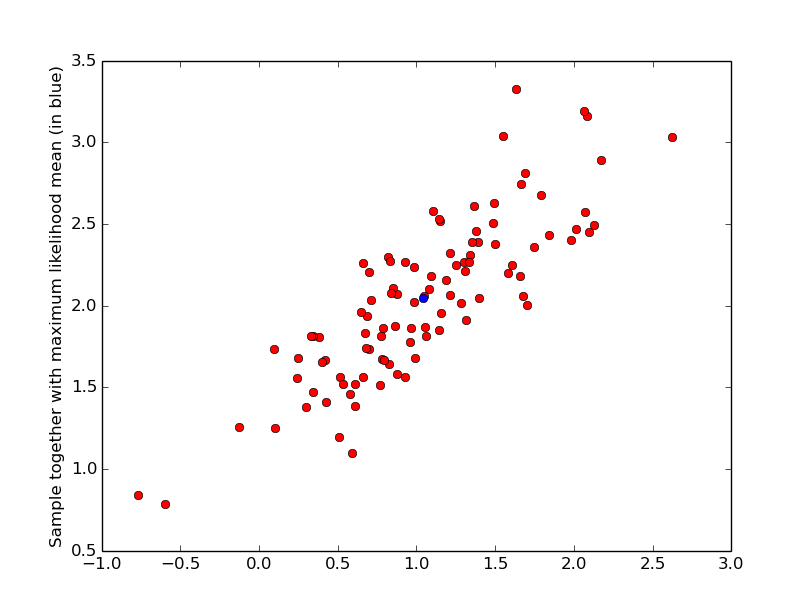
\includegraphics[width=.6\linewidth]{figures/samples_with_mean.png}
  \caption{Plot of the sample mean and the distribution mean together with the data set.}
  \label{fig:samples_with_mean}
\end{figure}

As shown in Figure~\ref{fig:samples_with_mean}, the Sample mean is $(1, 2)$ and the Distribution mean is $(1.06221568829, 2.00008779983)$ for an arbitrary execution. The Distribution mean deviates from the Sample mean since the generated data set only contains a hundred points. If the generated set were larger, the precision would increase, thus lowering the deviation between the Sample- and Deviation mean.

\subsection{Covariance: The Geometry of Multivariate Gaussian Distributions}
Figure~\ref{fig:samples_with_eigenvectors} shows the scaled and translated eigenvectors plotted on top of the sampled data set. As we saw in the lectures, the two eigenvectors represent the ``main directions'' of the covariance matrix (i.e., the directions of variance in the data set), and the eigenvalue represents the scale of the variance in the direction of the corresponding eigenvector.

\begin{figure}[H]
  \centering
  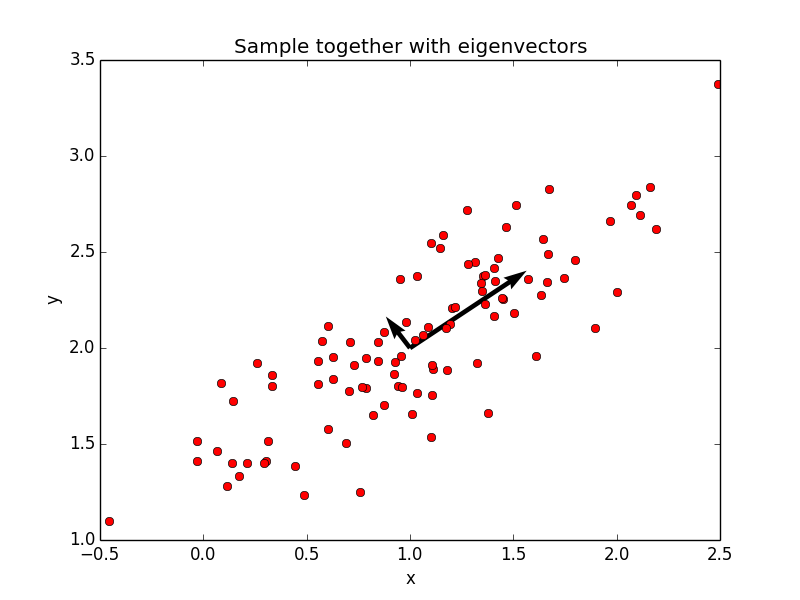
\includegraphics[width=.6\linewidth]{figures/samples_with_eigenvectors.png}
  \caption{Plot of the scaled and translated eigenvectors together with the data set.}
  \label{fig:samples_with_eigenvectors}
\end{figure}

Figure~\ref{fig:samples_rotated} shows samples from the rotated distributions for 30, 60 and 90 degree rotations of the covariance matrix. We have used the same randomly drawn z-values that generated the data set in I.2.2, so this is essentially the same data set as before, only rotated as we can see in the figure. Furthermore, the figure also the data set rotated by the angle $\phi$, computed as 43.9204246244 degrees in the depicted run, which causes the main direction of the data set to point along the $x$-axis of the figure. 

% Done: Find angle theta such that the main direction of the data points along the x axis.

\begin{figure}[H]
  \centering
  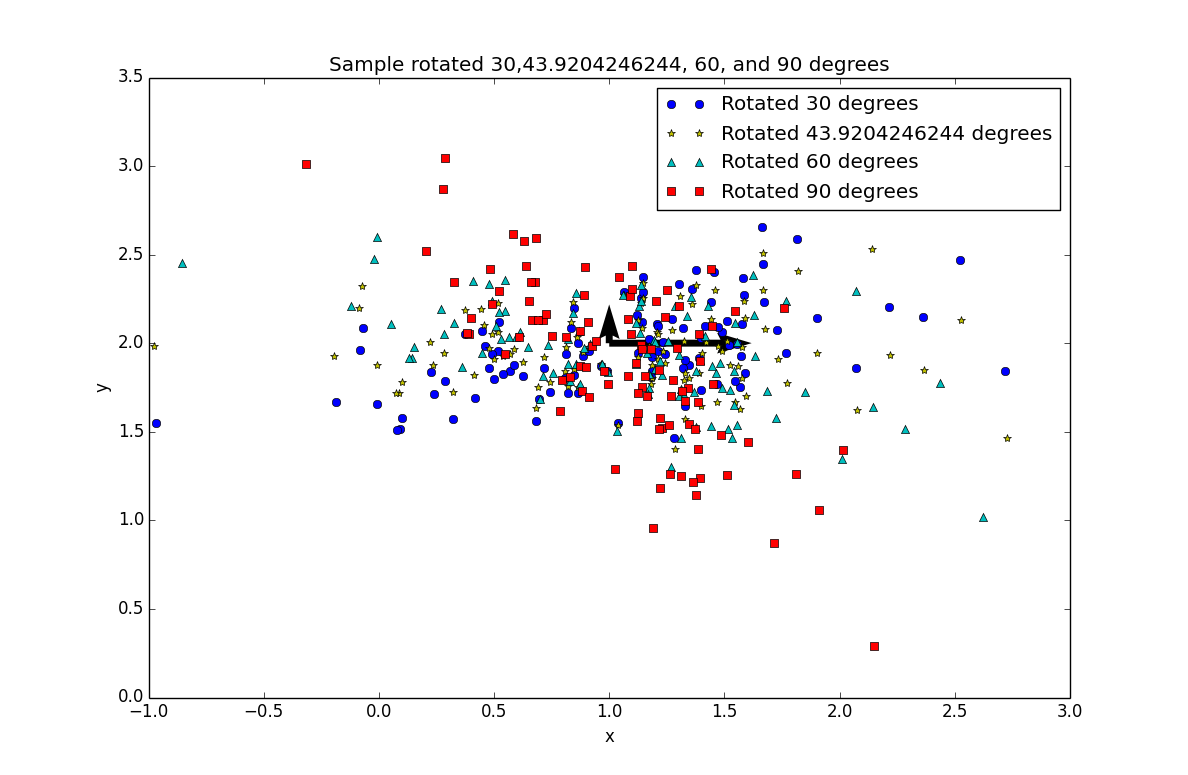
\includegraphics[width=1\linewidth]{figures/samples_rotated.png}
  \caption{Samples from the rotated distributions.}
  \label{fig:samples_rotated}
\end{figure}

\section{Classification}

\subsection{Nearest Neighbor}
Using the \texttt{IrisTrain2014.dt}-file as training data with the implemented $k$-NN classifier on the training and test data sets, the following accuracy results are obtained
\begin{figure}[H]
	\begin{lstlisting}
	Training set:
	K = 1: Accuracy = 1.0
	K = 3: Accuracy = 0.93
	K = 5: Accuracy = 0.85

	Test set:
	K = 1: Accuracy = 0.815789473684
	K = 3: Accuracy = 0.815789473684
	K = 5: Accuracy = 0.789473684211
	\end{lstlisting}
	\caption{Training and test results of the implemented $k$-NN classifier for $k=1,3,5$}
	\label{fig:k-nn_results}
\end{figure}

% TODO: Finish this argument
The classification of the training set with $k=1$ gives a $100\%$ as each data point is classified directly, as expected. As the $k$-value increases, the training set accuracy decreases as the number of neighbor-points increases, thus lowering the accuracy of the classification. For the test set, $k=1$ and $k=3$ give the same results. Increasing to $k=5$ decreases the accuracy which could indicate that the classification is quite sensitive to its surrounding neighbours.


\subsection{Hyperparameter Selection using Cross-validation}
The 5-fold cross validation was implemented in the form of an $N$-fold cross validation algorithm. The algorithm performs the cross validation by splitting an input training set into $N$ equally-sized parts, calculating the accuracy of each part with respect to the remaining parts and finally returning the mean of the calculated accuracies.\\

The hyperparameter selection suggested that the optimal number of neighbors were $k = 17$, as shown in figure~\ref{fig:5-fold_results}\\

The cross-validation implementation found $k_{best} = 17$ which upon estimating the performance using the test data resulted in an accuracy of $76\%$, as shown in figure \ref{fig:5-fold_results}. 

\begin{figure}[H]
	\begin{lstlisting}
	k = 1:  Validation-result = 0.84
	k = 3:  Validation-result = 0.85
	k = 5:  Validation-result = 0.83
	k = 7:  Validation-result = 0.84
	k = 9:  Validation-result = 0.86
	k = 11: Validation-result = 0.85
	k = 13: Validation-result = 0.86
	k = 15: Validation-result = 0.86
	k = 17: Validation-result = 0.87
	k = 19: Validation-result = 0.86
	k = 21: Validation-result = 0.86
	k = 23: Validation-result = 0.86
	k = 25: Validation-result = 0.86
	k_best = 17
	Training set: Accuracy = 0.87
	Test set: Accuracy = 0.763157894737
	\end{lstlisting}
	\caption{Accuracy for each $k$-value calculated by the implemented 5-fold cross validation}
	\label{fig:5-fold_results}
\end{figure}

\subsection{Data Normalization}


\begin{figure}[H]
	\begin{lstlisting}
	Training set, feature = 0: Mean = -3.46833672893e-15, variance = 1.0
	Training set, feature = 1: Mean = -1.81743509131e-15, variance = 1.0
	Test set, feature = 0: Mean = 0.208375768039, variance = 1.07339795338
	Test set, feature = 1: Mean = 0.432138257729, variance = 1.25222270424
	k = 1:  Validation-result = 0.78
	k = 3:  Validation-result = 0.69
	k = 5:  Validation-result = 0.72
	k = 7:  Validation-result = 0.72
	k = 9:  Validation-result = 0.71
	k = 11: Validation-result = 0.59
	k = 13: Validation-result = 0.62
	k = 15: Validation-result = 0.65
	k = 17: Validation-result = 0.65
	k = 19: Validation-result = 0.59
	k = 21: Validation-result = 0.57
	k = 23: Validation-result = 0.6
	k = 25: Validation-result = 0.64
	k_best = 1
	Training set: Accuracy = 1.0
	Test set: Accuracy = 0.789473684211
	\end{lstlisting}
	\caption{Mean, variances and accuracies of normalized data sets}
	\label{fig:normalization_results}
\end{figure}
\end{document}
